\section{Using other libraries}
\topics{Dependency management, using definitions from arbitrary libraries}

In \Cref{sec:lab-prelude}, we learnt how to create our own package and that Haskell's standard library, the \haskellIn{Prelude} module, is contained in the \texttt{\small base} package which we typically have as a dependency by default. When building real software, it is not unusual to have a significant number of dependencies, not just one. After all, it does not make sense for a team of software engineers to build everything from scratch -- instead it is a good idea to see what libraries other people have built already, there \emph{may}\footnote{Whenever you add an external dependency to a project you work on, you should use your judgement it is a good idea to do so in terms of the library's maturity, whether it is being maintained, and for possible security implications.} be more mature implementations of what you need already so there may be no need to invest time into building it again.

Haskell has a package repository called Hackage which you can search for Haskell packages:
\begin{center}\small
	\url{https://hackage.haskell.org/packages/search}
\end{center}
Alternatively to searching Hackage directly, you may also use Hoogle to search for functions and types across all indexed packages:
\begin{center}\small
	\url{https://hoogle.haskell.org}
\end{center}
When looking at the documentation for a module on Hackage, you can always see the name of the package (and the version) in the top left corner:
\begin{center}
	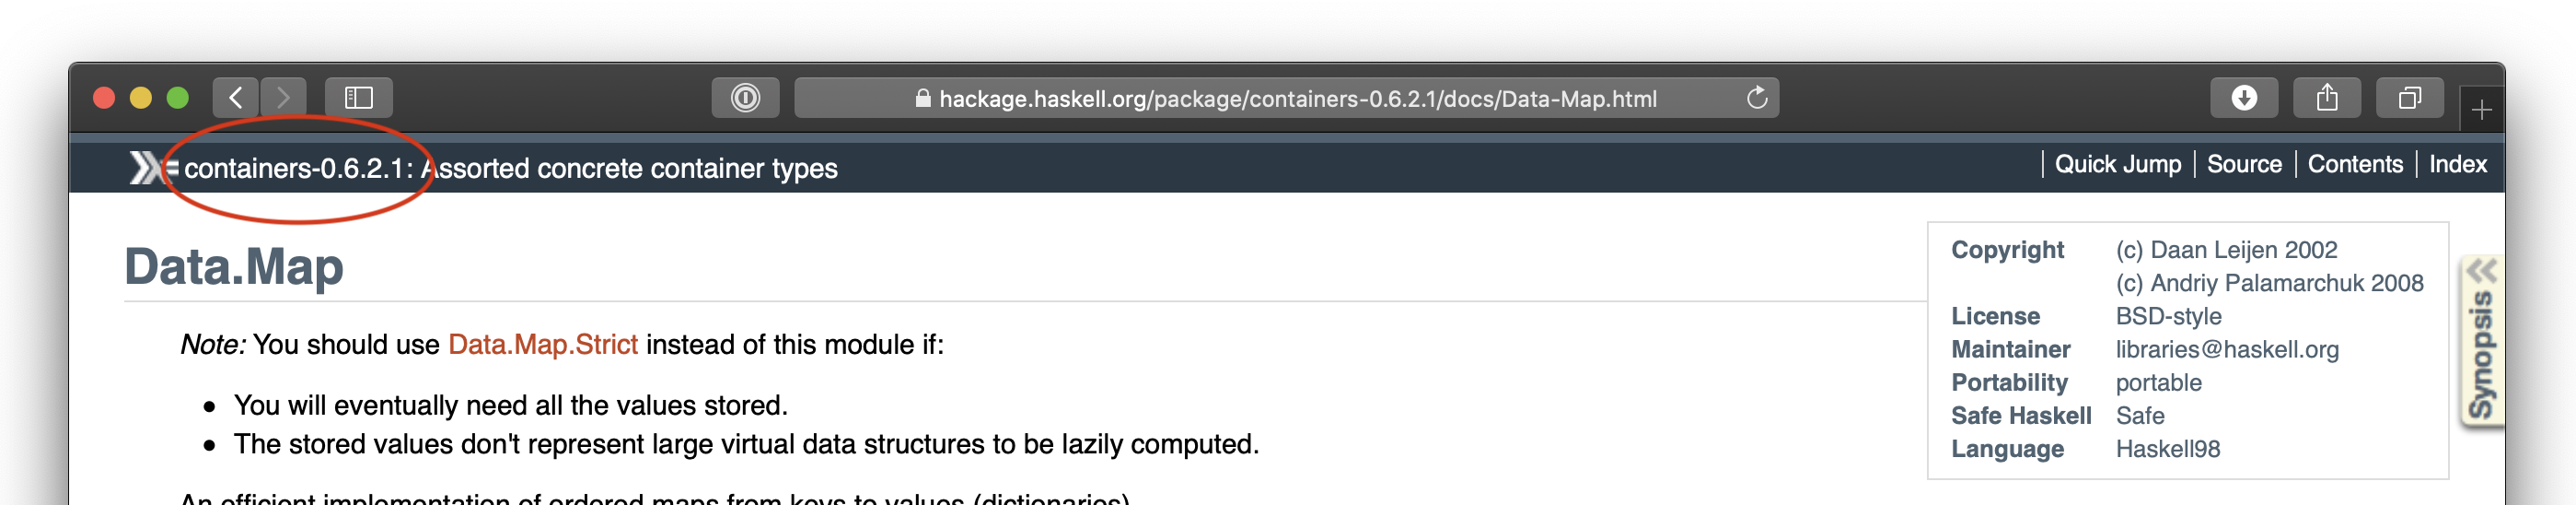
\includegraphics[width=\textwidth]{labs/hackage.png}
\end{center}
\emph{I.e.} to use the \haskellIn{Data.Map} module, you must add the \texttt{\small containers} package as a dependency to your project.

\makebox[0.5cm]{\faBook}~\emph{Recommended reading}: Chapter 7 of \emph{Learn you a Haskell} \citep{lipovaca2011learn}.

\paragraph{Stack resolver} Dependency management is actually quite a difficult problem because as we add more dependencies to a project, those dependencies may in turn have more dependencies, including with each other. This results in a \emph{dependency graph} where each edge is constrained by the version range that a package will accept for a particular dependency. In addition to being computationally difficult to solve all constraints, it is very easy for this to lead to unsatisfiable constraints if \emph{e.g.} multiple packages depend on different versions of another package. To improve on this situation, the \texttt{\small stack} tool has a notion of ``resolvers'' -- subsets of the Hackage package index in which all packages are known to be compatible with each other.

\taskLine 

\task{For this exercise, we will be creating another simple package from scratch with the help of \texttt{\small stack}. In a terminal, run the following:}
\begin{minted}{text}
$ stack new lab-dependencies simple-library --resolver=lts-16.27
\end{minted}

\task{Edit \texttt{\small lab-dependencies.cabal} to add a dependency to the \texttt{\small containers} package.}
\begin{minted}{text}
library
  -- ...
  build-depends:       base >= 4.7 && < 5, containers
\end{minted}
With this dependency added, you can now import any of the modules from the \texttt{\small containers} package:
\begin{center}\small
	\url{https://hackage.haskell.org/package/containers}
\end{center}
The \texttt{\small containers} package contains implementations of some data structures, including maps (dictionaries) and sets.

\task{Modify \texttt{\small src/Lib.hs} to import the \haskellIn{Data.Set} module, qualified as \haskellIn{S} to avoid clashes with names of functions in \haskellIn{Prelude}:}
\begin{minted}{haskell}
import qualified Data.Set as S
\end{minted}

\task{Add a definition to test that you can use functions and types imported from \haskellIn{Data.Set}:}
\begin{minted}{haskell}
set :: S.Set Int 
set = S.union (S.fromList [0..5]) (S.fromList [3..10])
\end{minted}
You may also wish to add \haskellIn{set} to the export list for the module (or remove the export list entirely to export everything automatically):
\begin{minted}{haskell}
module Lib (someFunc, set) where 
\end{minted}
Open the REPL with \texttt{\small stack repl} and evaluate \haskellIn{set} to check that the list you get as a result only contains every number once.